\chapter{Diagrammen}
\label{ch:Diagrammen}

\section{Android App Class Diagram}

In dit hoofdstuk zijn alle diagrammen terug te vinden met betrekking tot de gebruikte applicaties. Als eerste is het klassendiagram terug te vinden van de Android applicatie. Daarna het deployment diagram, en als laatste het ERD van Mongo. Van de MEAN stack kan niet echt een "klassen" diagram gemaakt worden aangezien dit een module based applicatie is en geen Object Oriented applicatie. De structuur zal beschreven worden als laatste punt.

\begin{figure}[H]
	\centering
	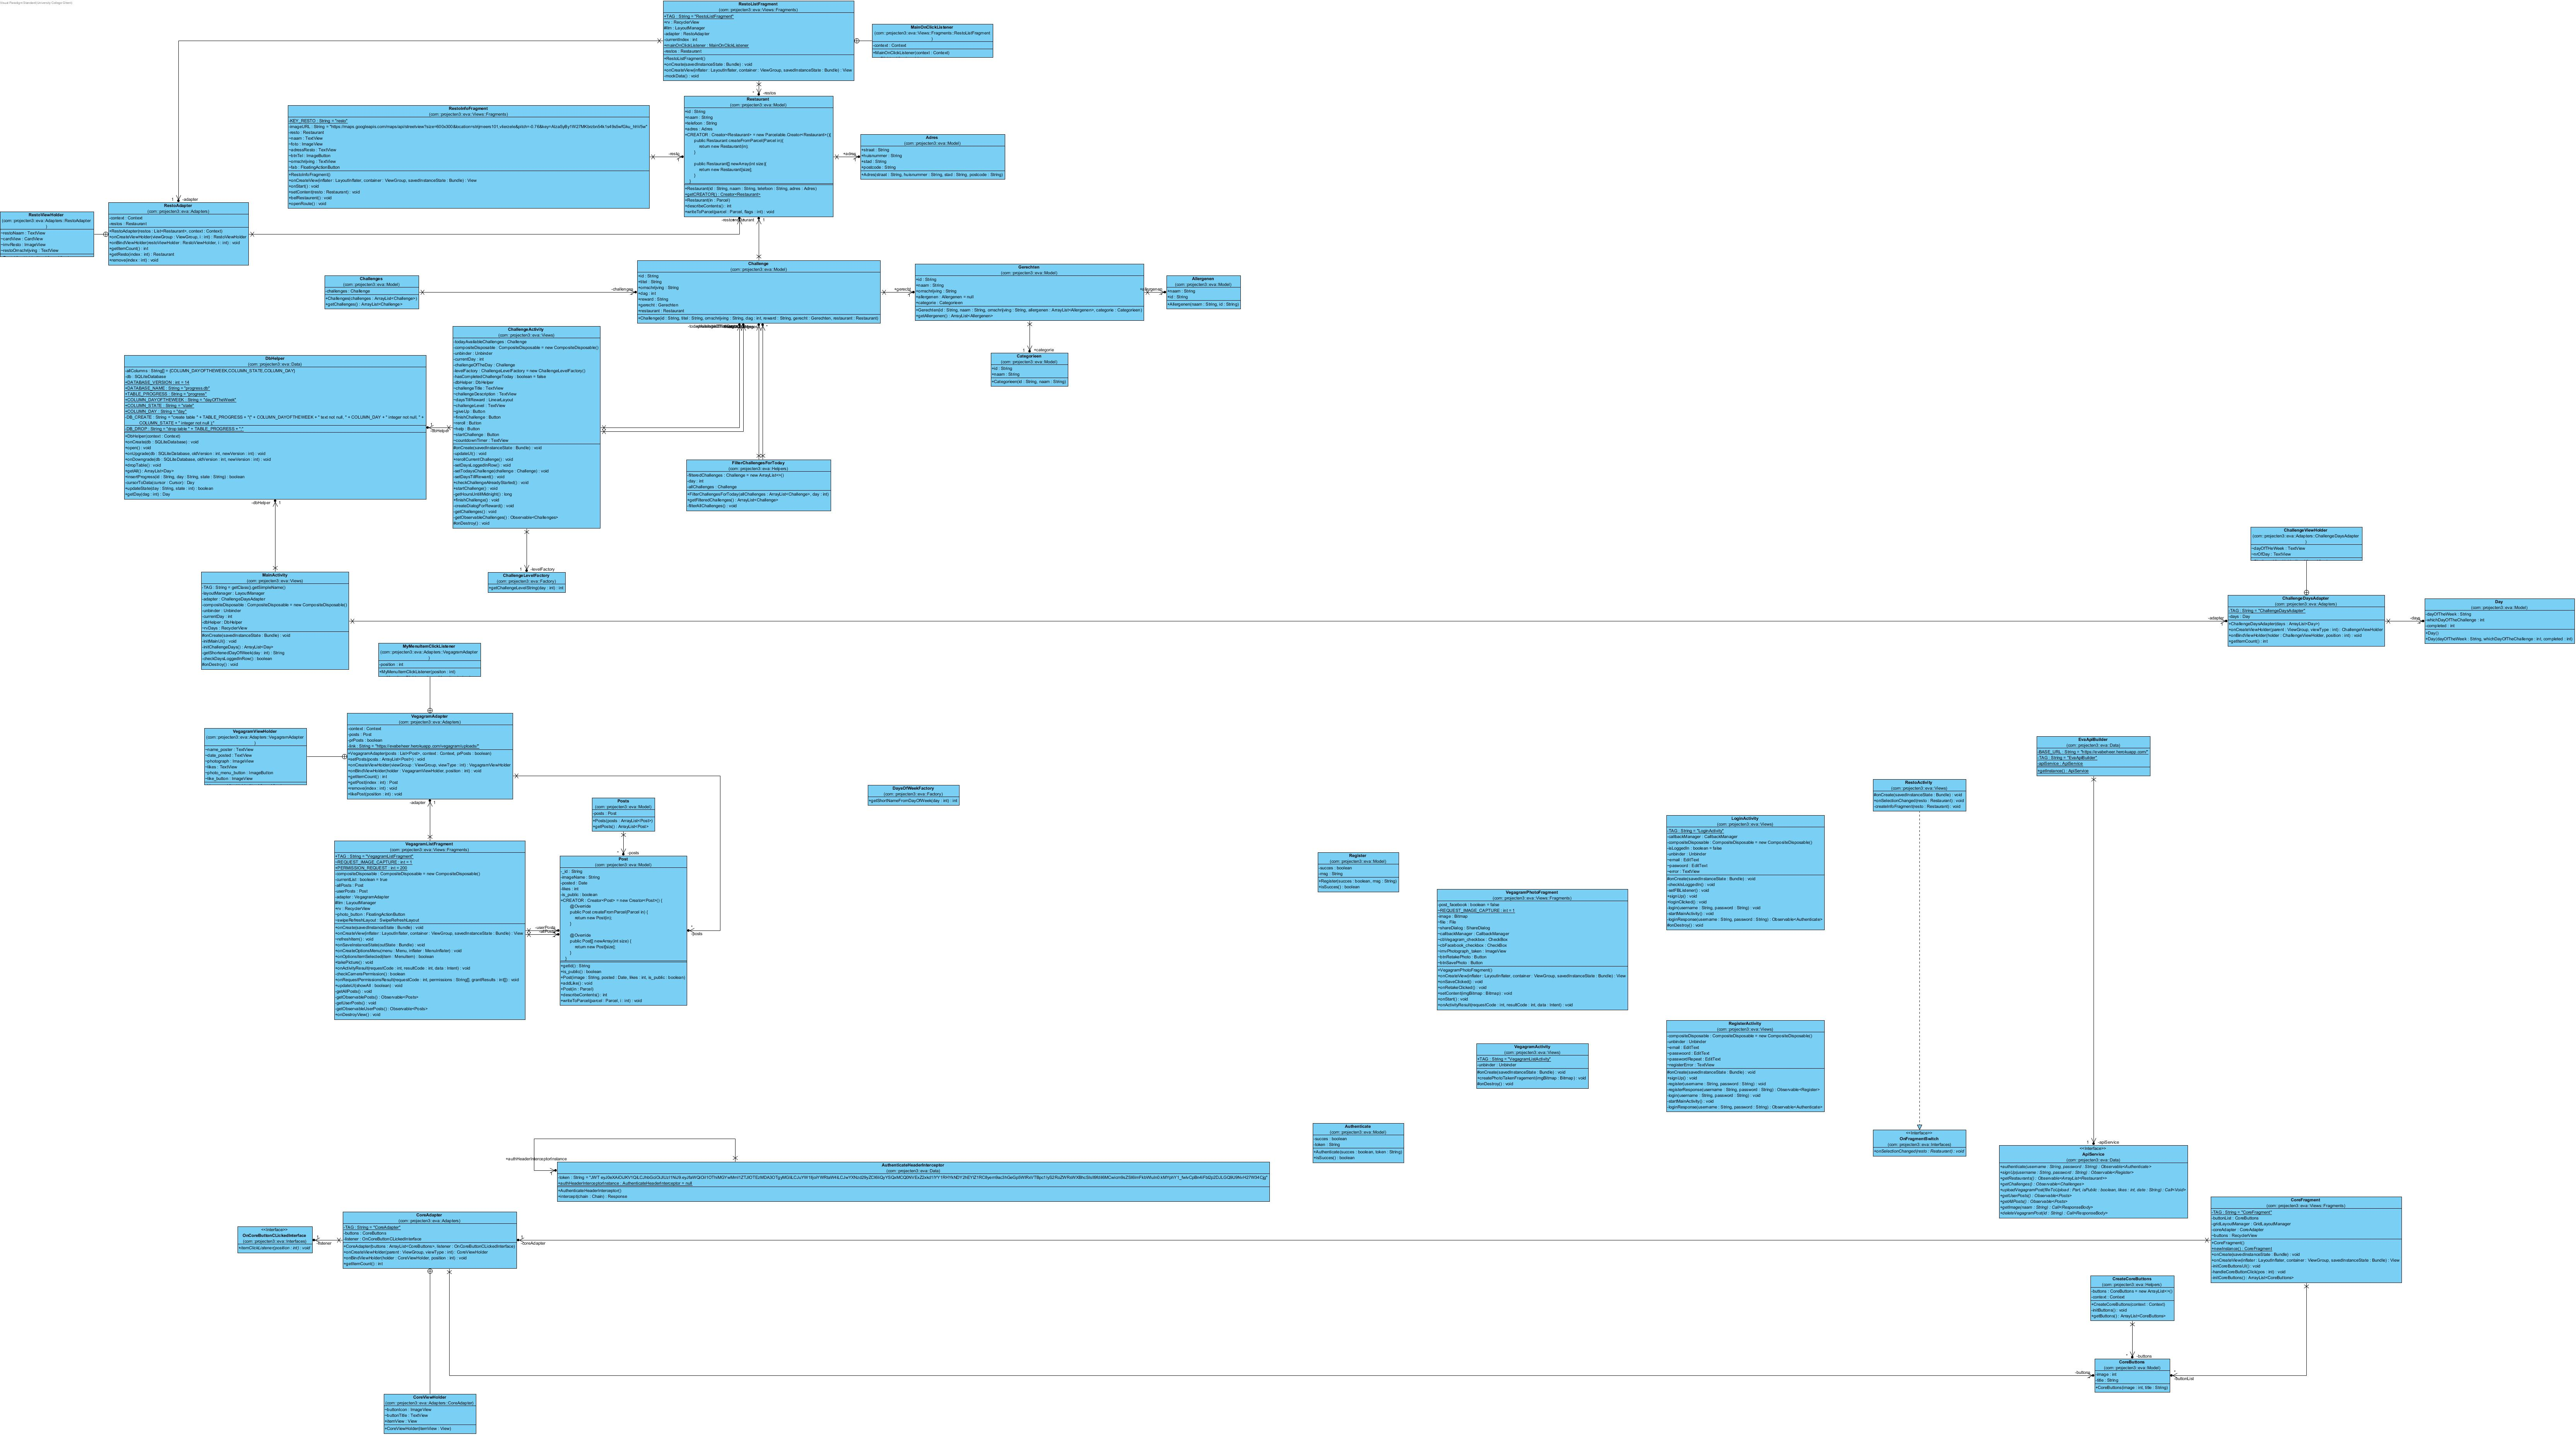
\includegraphics[width=10cm]{img/EvaAndroid.jpg}
	\caption{Eva Applicatie Class Diagram}
\end{figure}

een grote afbeelding is terug te vinden op de GitHub repository via volgende link: 

\section{Deployment Diagram}

Volgende afbeelding toont de deployment diagram aan van de workflow van zowel de Android applicatie als de MEAN applicatie.

\begin{figure}[H]
	\centering
	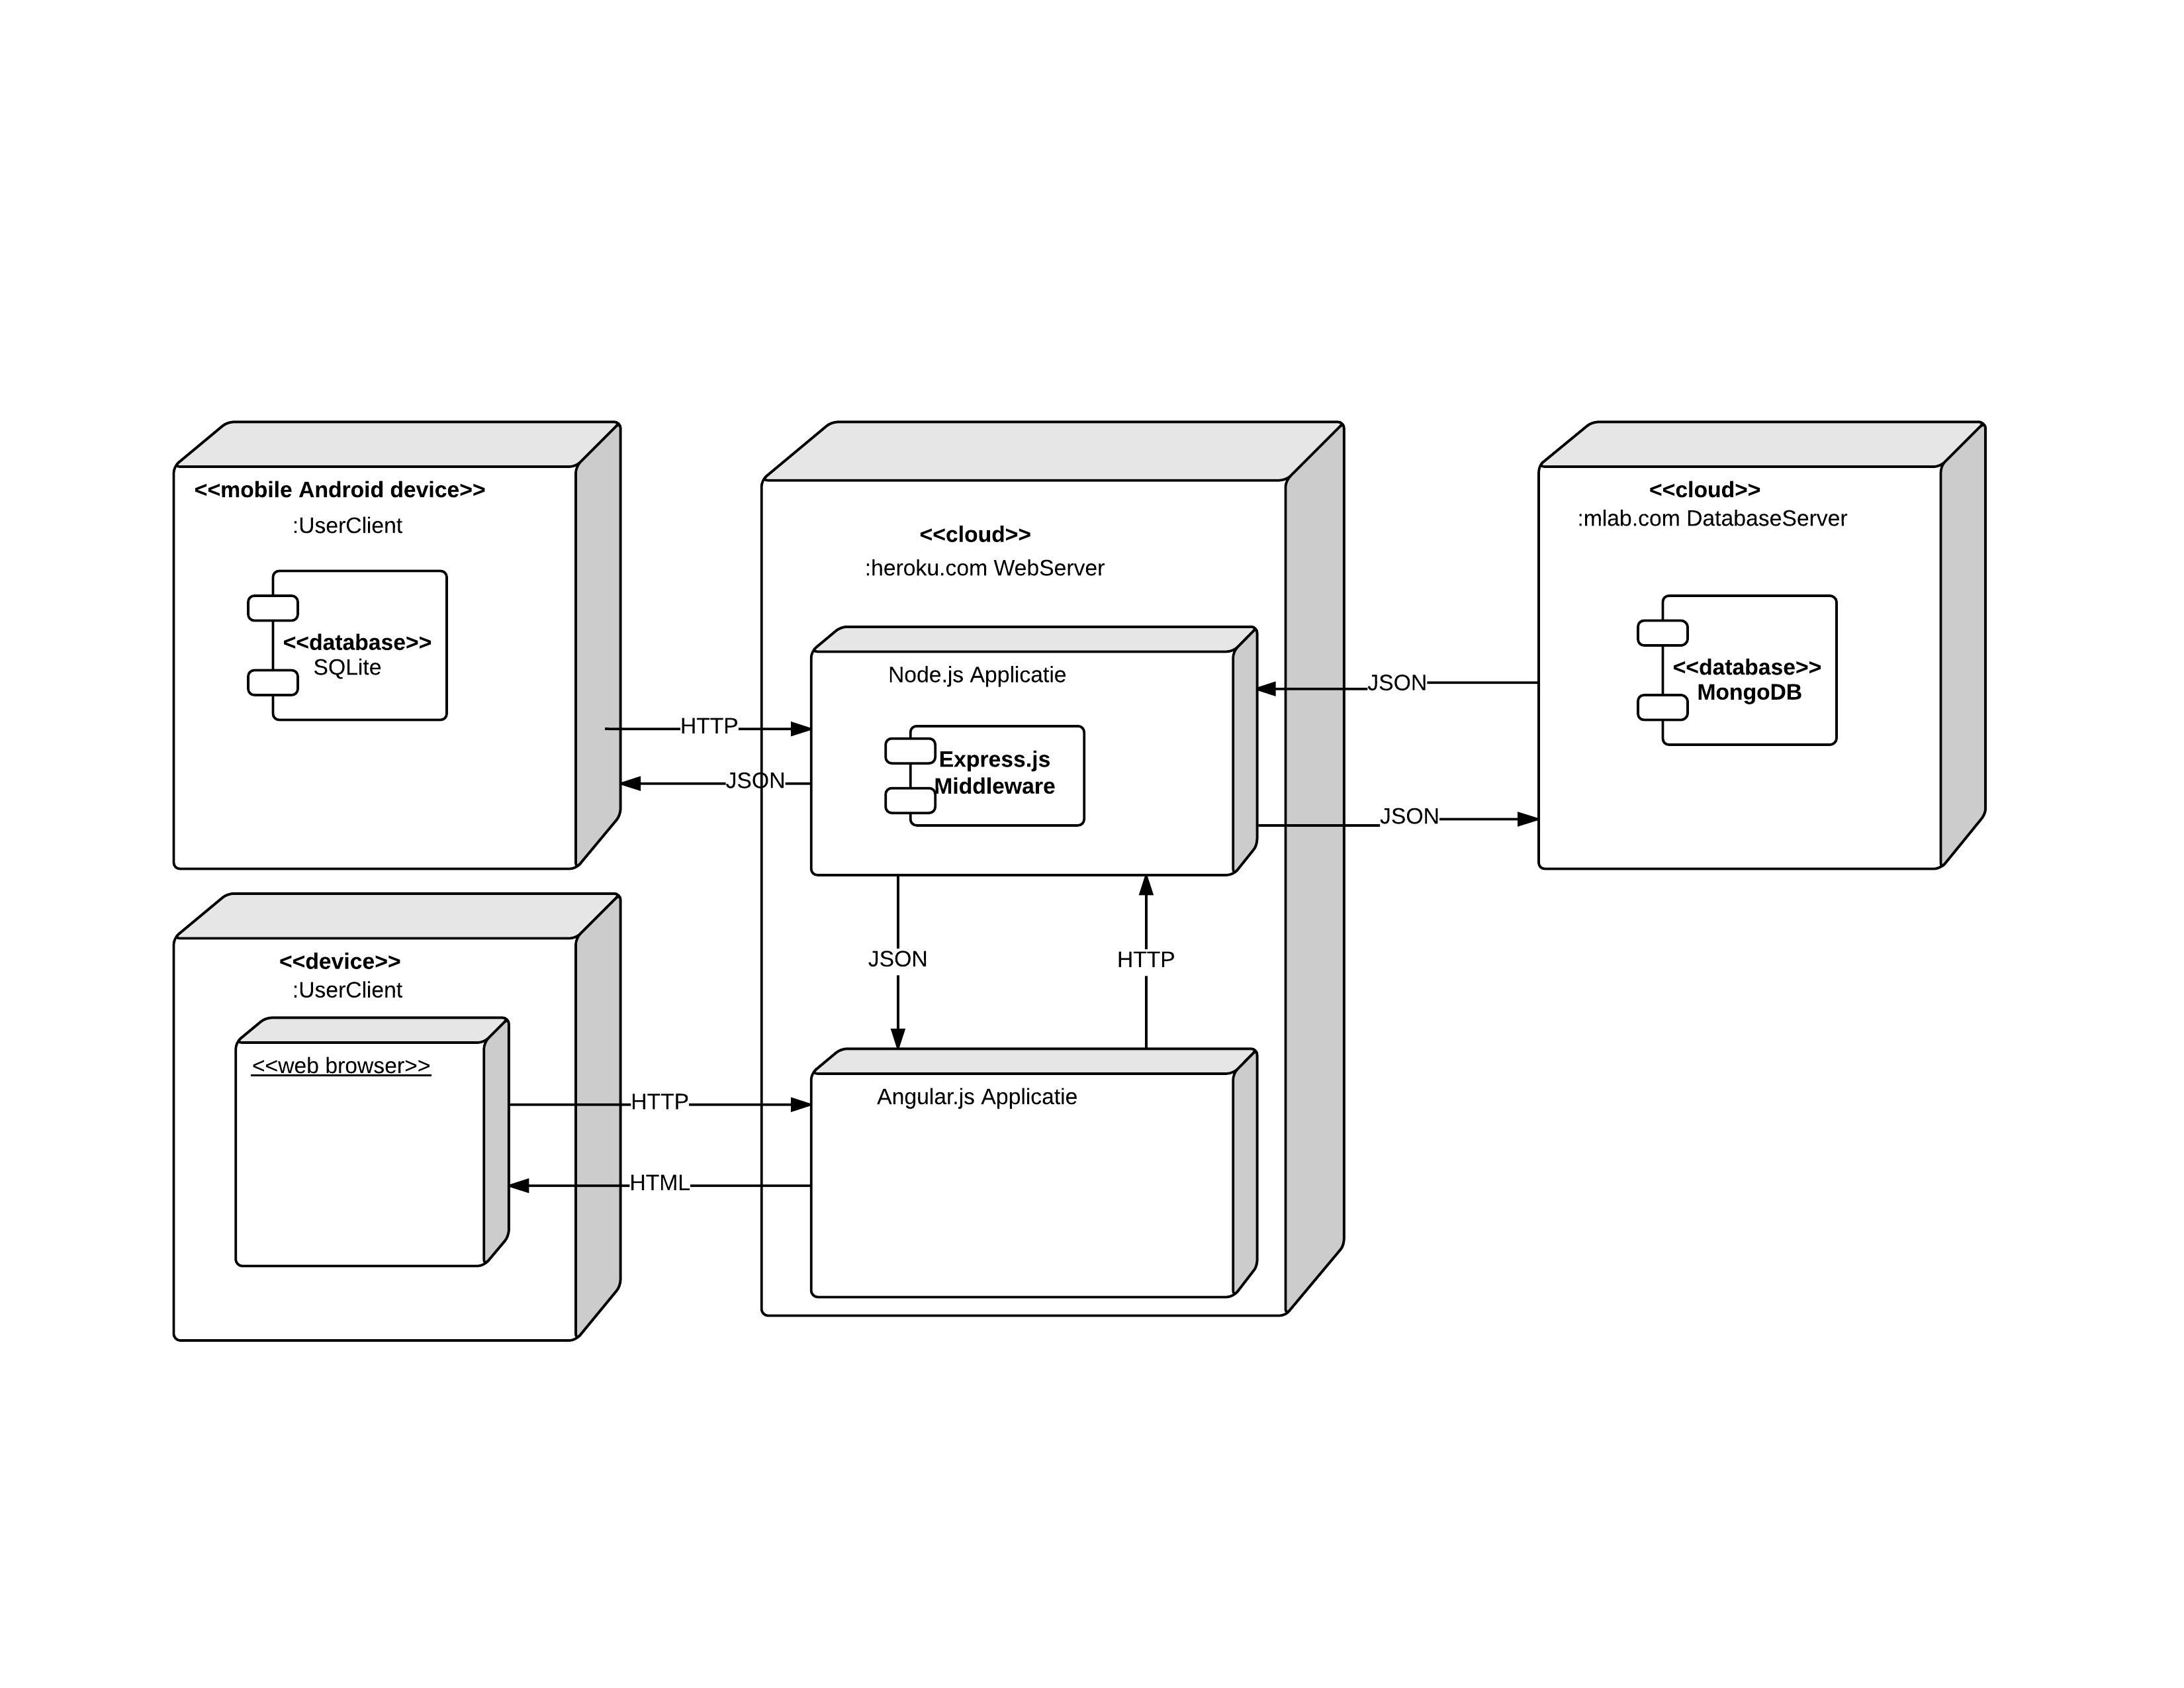
\includegraphics[width=15cm]{img/DeploymentDiagram.png}
	\caption{Deployment Diagram}
\end{figure}

\section{Entity Relationship Diagram}

De volgende afbeelding toont aan hoe het ERD er uit ziet. Waar aan duidelijk te zien is wat de databank van SQLite bevat, alsook de MongoDB.

\begin{figure}[H]
	\centering
	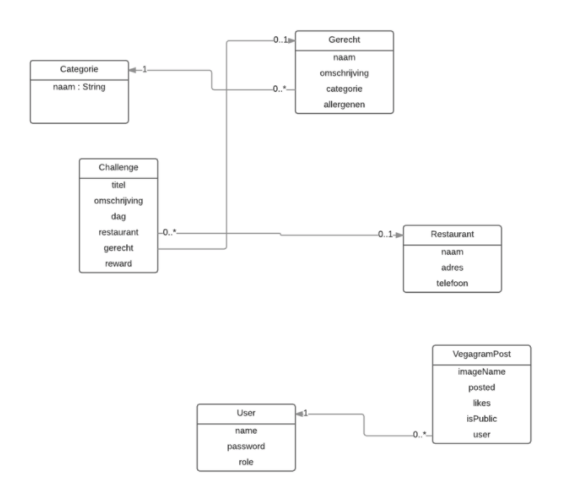
\includegraphics[width=15cm]{img/erd_mongo.png}
	\caption{Entitiy Relationship Diagram}
\end{figure}

De SQLite databank bevat maar één klasse die er als volgt uit ziet

\begin{figure}[H]
	\centering
	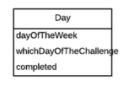
\includegraphics[width=5cm]{img/erd_sqlite.png}
	\caption{SQLite ERD}
\end{figure}

\section{Structuur MEAN}

De structuur van de MEAN applicatie bestaat uit de gevolgde best practices, zo hebben we volgende controllers

\begin{itemize}
\item RestaurantDetailModalController
\item RestaurantModalController
\item authController
\item categorieModalController
\item challengeController
\item challengeDetailModalController
\item challengeModalController
\item gerechtDetailModalController
\item gerechtModalController
\item restauransController
\end{itemize}

Deze maken gebruik van de volgende Factories en services


\begin{itemize}
	\item authService
	\item beheer-factory
	\item challenge-factory
	\item restaurants-factory
\end{itemize}

Dit alles werkt samen om alles te genereren dat getoond wordt in de html van de volgende pagina's

\begin{itemize}
	\item allergenen
	\item categorieen
	\item challenges
	\item gerechtBeheer
	\item restaurants
\end{itemize}

en volgende modals


\begin{itemize}
	\item categorieModal
	\item challengeDetailModal
	\item challengeModal
	\item gerechtenDetailModal
	\item gerechtModal
	\item restaurantModal
	\item restaurantDetailModal
\end{itemize}


